\subsection*{Уширение спектральных линий}

\subsubsection*{Естественная ширина линии}

В нашем случае это квантовое определение, которому мы прикрутим классические колёса. А именно, возьмём модель осциллятора, то есть атом излучает как:
\begin{equation*}
	\ddot{x} + 2 \gamma \dot{x} \omega_0^2 x = 0,
	\hspace{0.5 cm}
	x(0) = x_0,
	\hspace{0.5 cm}
	\dot{x}(0) = 0.
\end{equation*}
И решение соответственно:
\begin{equation*}
	x(t) = x_0 e^{- \gamma t} (\cos \omega t +\frac{\gamma}{2 \omega}\sin \omega t),
	\hspace{0.5 cm}
	\omega = \sqrt{\omega_0 - \gamma^2}.
\end{equation*}
Будем считать, что затухание у нас слабое:
\begin{equation*}
	\gamma << \omega_0 
	\hspace{0.6 cm}
	\Rightarrow
	\hspace{0.6 cm}
	x(t) = x_0 e^{-\gamma t} \cos \omega_0 t.
\end{equation*}
\begin{equation*}
	x(t) = \frac{1}{\sqrt{2 \pi}} \int_{-\infty}^{+\infty} A(\omega) e^{i \omega t} d\omega,
	\hspace{0.5 cm}
	A(\omega) = \frac{1}{\sqrt{2 \pi}} \int_{-\infty}^{+\infty} x(t) e^{-i \omega t}d t.
\end{equation*}
Имеем итого "амплитуду" преобразования Фурье:
\begin{equation*}
	A(\omega) = \frac{1}{\sqrt{2 \pi}} \int_{-\infty}^{+\infty} x_0 e^{-\gamma t} \cos \omega_0 t e^{-i \omega t}d t
	=
	\frac{1}{2\sqrt{2 \pi}} \int_{0}^{+\infty} x_0 e^{-\gamma t} e^{i(\omega_0 - \omega)t} d t
	+
	\frac{1}{2\sqrt{2 \pi}} \int_{0}^{+\infty} x_0 e^{-\gamma t} e^{i(\omega_0 + \omega)t} d t = 
\end{equation*}
\begin{equation*}
	= \frac{x_0}{2 \sqrt{2 \pi}}
	\left(
	\frac{e^{- \gamma t + i (\omega_0 - \omega)t}}{i (\omega_0 - \omega) - \gamma}
	+
	\underbrace{\frac{e^{- \gamma t + i (\omega_0 + \omega)t}}{i (\omega_0 + \omega) - \gamma}}_{\to 0}
	\right)
	\bigg|_0^\infty = \frac{x_0}{2 \sqrt{2\pi} (i (\omega_0 - \omega) - \gamma)}.
\end{equation*}
Но узнавать что-то мы ведь можем только про интесивнсоть:
\begin{equation*}
	I = \frac{x_0^2}{8 \pi ( (\omega_0 - \omega)^2 + \gamma^2 )}.
\end{equation*}
Ширина профиля $I(\omega))$ порядка $10^9$.

\subsubsection*{Доплеровское уширение}
При движении детектируемого источника на/от вас фиксируемая частота будет:
\begin{equation*}
	\omega = \omega_0 \left(1 + \frac{v_x}{c}\right)
	\hspace{1 cm}
	\Rightarrow
	\hspace{1 cm}
	\omega = \omega_0 (1 + \vc{k} \cdot \vc{v}).
\end{equation*}
То есть сколько-то атомов летит с одной скоростью на вас, сколько-то перепендикулярно вам но с большей скорости. Таким образом имеет место Гауссово распределение этих атомов по скоростям. Соотвественно больше всего тех, кто вообще не движется в проекции на вашу ось.
\begin{figure}[h]
    \centering
    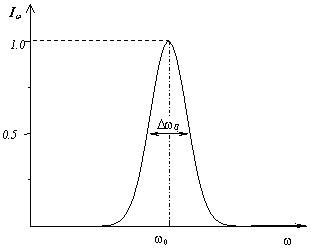
\includegraphics[width=0.3\textwidth]{img/ushir.jpg}
    %\caption{}
    %\label{fig:}
\end{figure}


Поговорим теперь про распределения:
\begin{equation*}
	v_0^2 = \frac{2 r T }{m}
	\hspace{1 cm}
	\Rightarrow
	\hspace{1 cm}
	d N =  N \exp\left( - \frac{(\omega - \omega_0)^2 c^2}{\omega_0^2 v_0^2}\right)\frac{c}{\omega_0} d \omega.
\end{equation*}

\subsubsection*{Столкновительное уширение}
\subsubsection*{Времяпролётное уширение}

\subsection*{Внутридоплеровская сперктроскопия}
\textbf{Постановка задачи:} есть атомы в коробку, которые носятся туда-сюда, а мы такие берём и посылаем пучок (ну или следим за пучок оттуда). Пусть мы нашли две линии, но из-за доплеровского уширения, если линии близки, то они неплохо так сольются, и различить их будет трудно.
\begin{figure}[h]
    \centering
    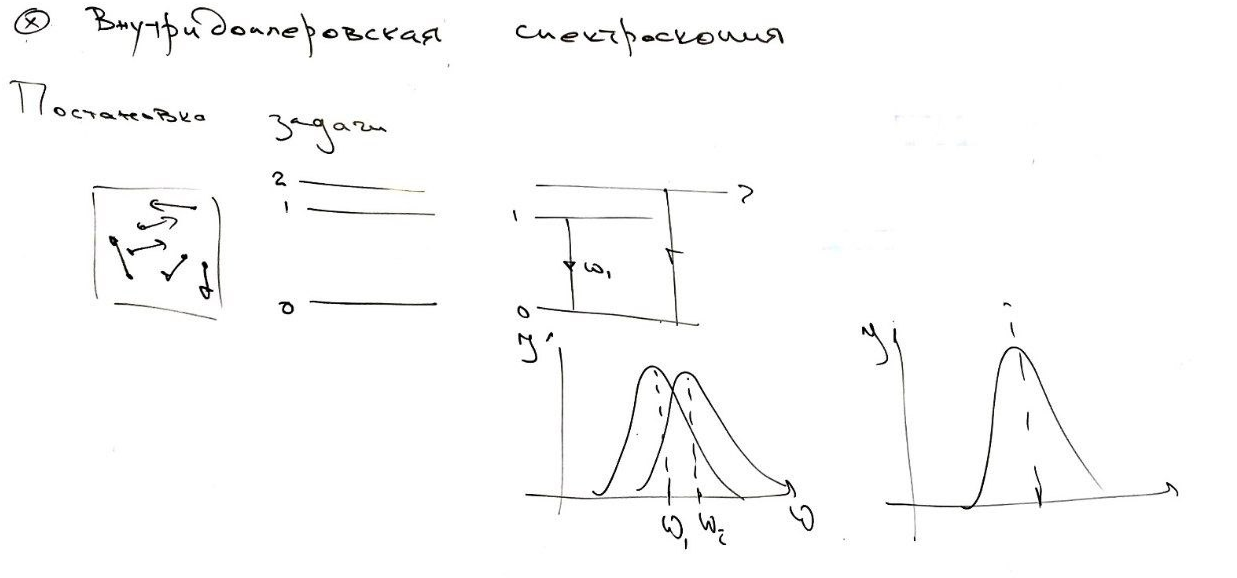
\includegraphics[width=0.7\textwidth]{img/lec_6.png}
    %\caption{}
    %\label{fig:}
\end{figure}

\subsubsection*{Квантовая механика для самых маленьких: что умеет делать электрон?}
Для сечения $\sigma$ (вероятность что-то сделать) про переходы электронов на уровни вних под/без действия внешнего излучения ответ:
\begin{itemize}
	\item электрон умеет поглощать фотончик $h \nu$;
	\item электрон умеет вынужденно излучать;
	\item электрон умеет спонтанно излучать;
	\item электрон умеет не излучать.
\end{itemize}
 
\subsubsection*{Кинематические уравнения (скоростные)}
Для двух уравнений, количество электронов на уровне: $n_1$ и $n_2$. Для характерных времен b -- bезизлучательного процесса и с -- спонтанного процесса.
\begin{equation*}
	\dot{n}_2 = - \frac{n_2}{\tau_b} - \frac{n_2}{\tau_c}
	\hspace{1 cm}
	\Rightarrow
	\hspace{1 cm}
	n_2 = n_{2 0 } \exp\left(- \frac{t}{\tau_b} - \frac{t}{\tau_c}\right).
\end{equation*}
Если есть поток фотонов $F = \frac{I}{h\nu}$, который побуждает переходить электроны и с верхнего не нижний и наоборот:
\begin{equation*}
	\dot{n}_1 = - F \sigma n_1 + F \sigma n_2 +\frac{n_2}{\tau_b}.
\end{equation*}
\begin{equation*}
	\dot{n}_2 = F \sigma n_1 - F \sigma n_2 -\frac{n_2}{\tau_b}.	
\end{equation*}
Для $n_1 + n_2 = N$:
\begin{equation*}
	\dot{n}_1 = - F \sigma n_1 + F \sigma n_2 +\frac{n_2}{\tau_b} + \frac{N}{\tau_b} - \frac{n_1}{\tau_b}
	\hspace{0.5 cm}
	\Rightarrow
	\hspace{0.5 cm}
	\dot{n}_1 + n_1 \left(2 \sigma F + \frac{1}{\tau_b}\right) = N \sigma F + \frac{N}{\tau_b}.
\end{equation*}
Таким образом:
\begin{equation*}
	n_1 = N \frac{\sigma F + \frac{1}{\tau_b}}{2 \sigma F + \frac{1}{\tau_b}} = N \frac{F + \frac{1}{`s \tau_b}}{2 F + \frac{1}{\sigma \tau_b}}.
\end{equation*}
А теперь если сказать, что то, сколько приходит и сколько уходит равны, потому как просто больше некому излучаться и поглощать, то:
\begin{equation*}
	0 = - n_1 \sigma F + n_2 \sigma F + \frac{n_2}{\tau_b}
\end{equation*}
Обозначим как что-то характерное $F_s = \frac{1}{\gamma \tau_b}$, тогда имеем 
\begin{equation*}
	n(F) = N \frac{F + F_s}{2 F + F_s}.
\end{equation*}
И введем ещё такую величину на веру: коэффициент поглощения --- $\alpha = n_1 \sigma - n_2 \sigma$. Почему так удобно:
\begin{equation*}
	d F = - (n_1 \sigma - n_2 \sigma) F d z.
\end{equation*}

Наконец. Если есть среда, которая, например поглощает красный свет, но мы будем всё больше увеличивать падающий поток, то рано или поздно атомов не хватит на поглощене и материал \textit{просветлиться}.
\begin{figure}[h]
    \centering
    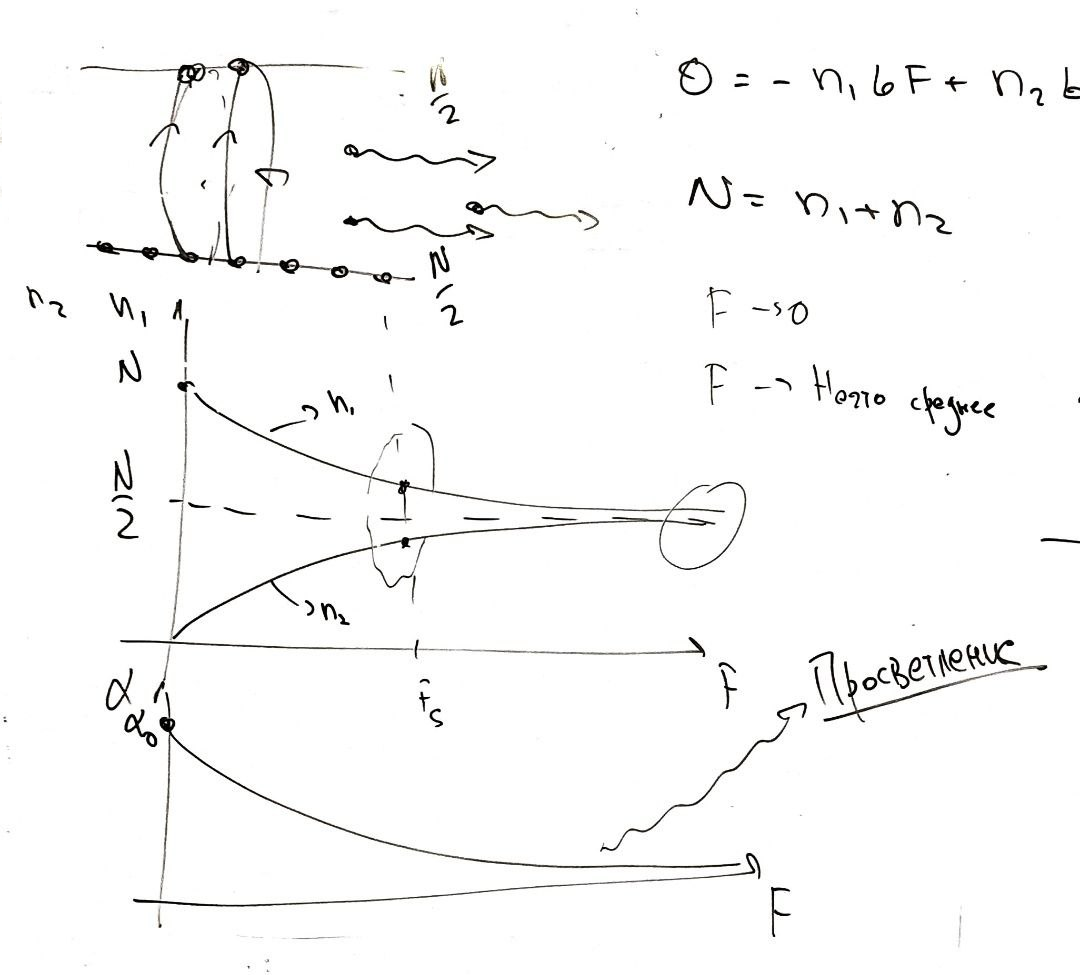
\includegraphics[width=0.4\textwidth]{img/lec_6_zerg.png}
    %\caption{}
    %\label{fig:}
\end{figure}


Напрягаемся в последний раз. Много слушаем и узнаем про провал Лэмба.